\title{Using RNN to Predict Stock Market Prices}
\author{Ford Smith}
\date{\today}

\documentclass[12pt]{article}

\usepackage{xcolor}
\usepackage{graphicx}
\usepackage{float}
\usepackage{booktabs}

\begin{document}
\maketitle

\begin{abstract}
\color{red} //TODO
\end{abstract}

\section{Introduction}
\quad When most people talk about Artificial Intelligence, they are describing machine learning. Machine learning has several difference subsections of tools that can be used to teach a machine from previous experiences by adjusting to inputs to ``perform human-like tasks" (SAS). In this particular experiment, Neural Networks will be used. Neural Networks are very powerful tools because they grant flexibility to many different scenarios depending on how they are constructed. 


\paragraph{History}
At its core, machine learning is all about taking in inputs and creating a generalized function that can then be extended to predict future values. In fact, humans have been doing basic variations of this for hundreds of years: linear regressions. While some function are too difficult to create, a line of best fit can be found on data with an input (x) and output (y) to create a function that can approximate or predict a different set of data. See Figure 1. 
%http://www.andreykurenkov.com/writing/ai/a-brief-history-of-neural-nets-and-deep-learning/

\begin{figure}[H]
    \centering
    \def\svgwidth{\columnwidth}
    \input{LinearRegression.pdf_tex}
    \caption{An example of linear regression used on input data to create a function to approximate more data}
\end{figure}

This type of learning is called supervised machine learning because through the process of approximating the function, input and output data can be used to make the approximation much more accurate. Unsupervised learning, although not important in this experiment, is learning where there are not output values so different learning methods are used to learn more about the inputs and how it is structured. \\%https://machinelearningmastery.com/supervised-and-unsupervised-machine-learning-algorithms/

%http://www.andreykurenkov.com/writing/ai/a-brief-history-of-neural-nets-and-deep-learning/
Skip forward about 150 years to the 1950s, there is the development of the Perceptron. The Perceptron was created by Frank Rosenblatt to be a mathematical model of the neurons in our brains. It takes a set of inputs from nearby Perceptrons, multiplies each of the inputs by a valued weight, and will output a 1 if the weighted inputs reach a threshold, otherwise a 0. This was massive back then because Perceptrons could create basic OR/AND/NOT functions. This was the gateway to formal logic for computers. The most exciting part, however, was that this model could learn by slightly adjusting the weights whenever the output is too low/high. It followed this general order: "
\begin{enumerate}
\item Start off with a Perceptron having random weights and a training set
\item For the inputs of an example in the training set, compute the Perceptron’s output
\item If the output of the Perceptron does not match the output that is known to be correct for the example: If the output should have been 0 but was 1, decrease the weights that had an input of 1. If the output should have been 1 but was 0, increase the weights that had an input of 1.
\item Go to the next example in the training set and repeat steps 2-4 until the Perceptron makes no more mistakes"
\end{enumerate}

This procedure is simple, not terribly computationally heavy, and works best when there is only a limited set of outputs due to thresholds. This is exactly what classification requires - out of a set, accurately determine which output the input data is. Rosenblatt implemented the Perceptrons and inputted 20x20 inputs to accurately classify shapes. Although simple, when many Perceptrons are put together in series called \textbf{layers}, the computation power becomes much higher and can work on much more complex data. The same happens with multiple layers, where data is put into the input layer, which feeds their output to "hidden" layers who pass their information on to another layer until the information is passed to an output layer. The importance of these hidden layers stems from their ability to find features within the data. Features are essentially specific parts about the data passing through. For instance, if the network was trained to identify whether there was a cat in the image, the layer could identify whether the image has a cat mouth or not. This, in turn, allows it to become more accurate. However, there becomes several serious issues when done. First, Rosenblatt's method of training does not work with multiple layers. The Perceptrons also can't work on complex features because of the extreme linearity of the weight function inside the Perceptrons. 

%http://neuralnetworksanddeeplearning.com/chap2.html
%http://neuralnetworksanddeeplearning.com/chap1.html
\paragraph{Modern Networks}
\textbf{Backpropagation} was developed across multiple researchers in the 60s and is still commonly used. To break down what backpropagation is, is there is a cost function $C$ with respect to the weights $w$ in the network. Take the partial derivative of $C$ in respect to $w$ to then see how quickly the cost changes when the weights change. The reason backpropagation is so important was because it not only became a much faster learning algorithm, but also describes detailed information about the change in the system in respect to the weights.  \\

With a newer, faster, and all around better learning algorithm, there is still bottle-necking by the actual Perceptron itself. When there is a tiny change in its weights, it could cause a drastic change in the output, which actually makes training more difficult. If there is more fine control of the weights to have more fine control over the output, it is possible to more accurately train layers to get the results desired. This is where the sigmoid function comes in handy. If the threshold is replaced with the sigmoid function, as pictured below, there will be more fine change in the output with the change in the weights, giving a higher degree of accuracy.

\begin{figure}[H]
    \centering
    \def\svgwidth{\columnwidth}
    \input{Sigmoid.pdf_tex}
    \caption{An example of a sigmoid function}
\end{figure}

You may be wondering, why use the sigmoid function instead of just having the threshold? Well, the threshold is very linear and doesn't give much opportunity to learn around the data. When the \textbf{activation function} is non-linear (like the sigmoid function) it allows the network as a whole to better adapt to the data. Note, the activation function is what is used to determine the output of the nodes. Here is an image of what a complete Neural Network will use as Figure 3.

%https://medium.com/@curiousily/tensorflow-for-hackers-part-iv-neural-network-from-scratch-1a4f504dfa8
\begin{figure}[H]
  \includegraphics[width=\linewidth]{images/nn.png}
  \caption{A neural network}
\end{figure}

\section{Different Types}
%https://www.analyticsindiamag.com/6-types-of-artificial-neural-networks-currently-being-used-in-todays-technology/
\quad With the basics of what a neural network is and how it developed, it is important to cover the different types of Neural Networks - which will now just be referred to as NN - to best decide which will be used for this experiment. You will understand which one will be chosen and why it is the only one that can work in a moment. The main types are demonstrated in a graphic by Fjodor van Veen from Asimov Institute. 

%https://towardsdatascience.com/the-mostly-complete-chart-of-neural-networks-explained-3fb6f2367464
\begin{figure}[H]
  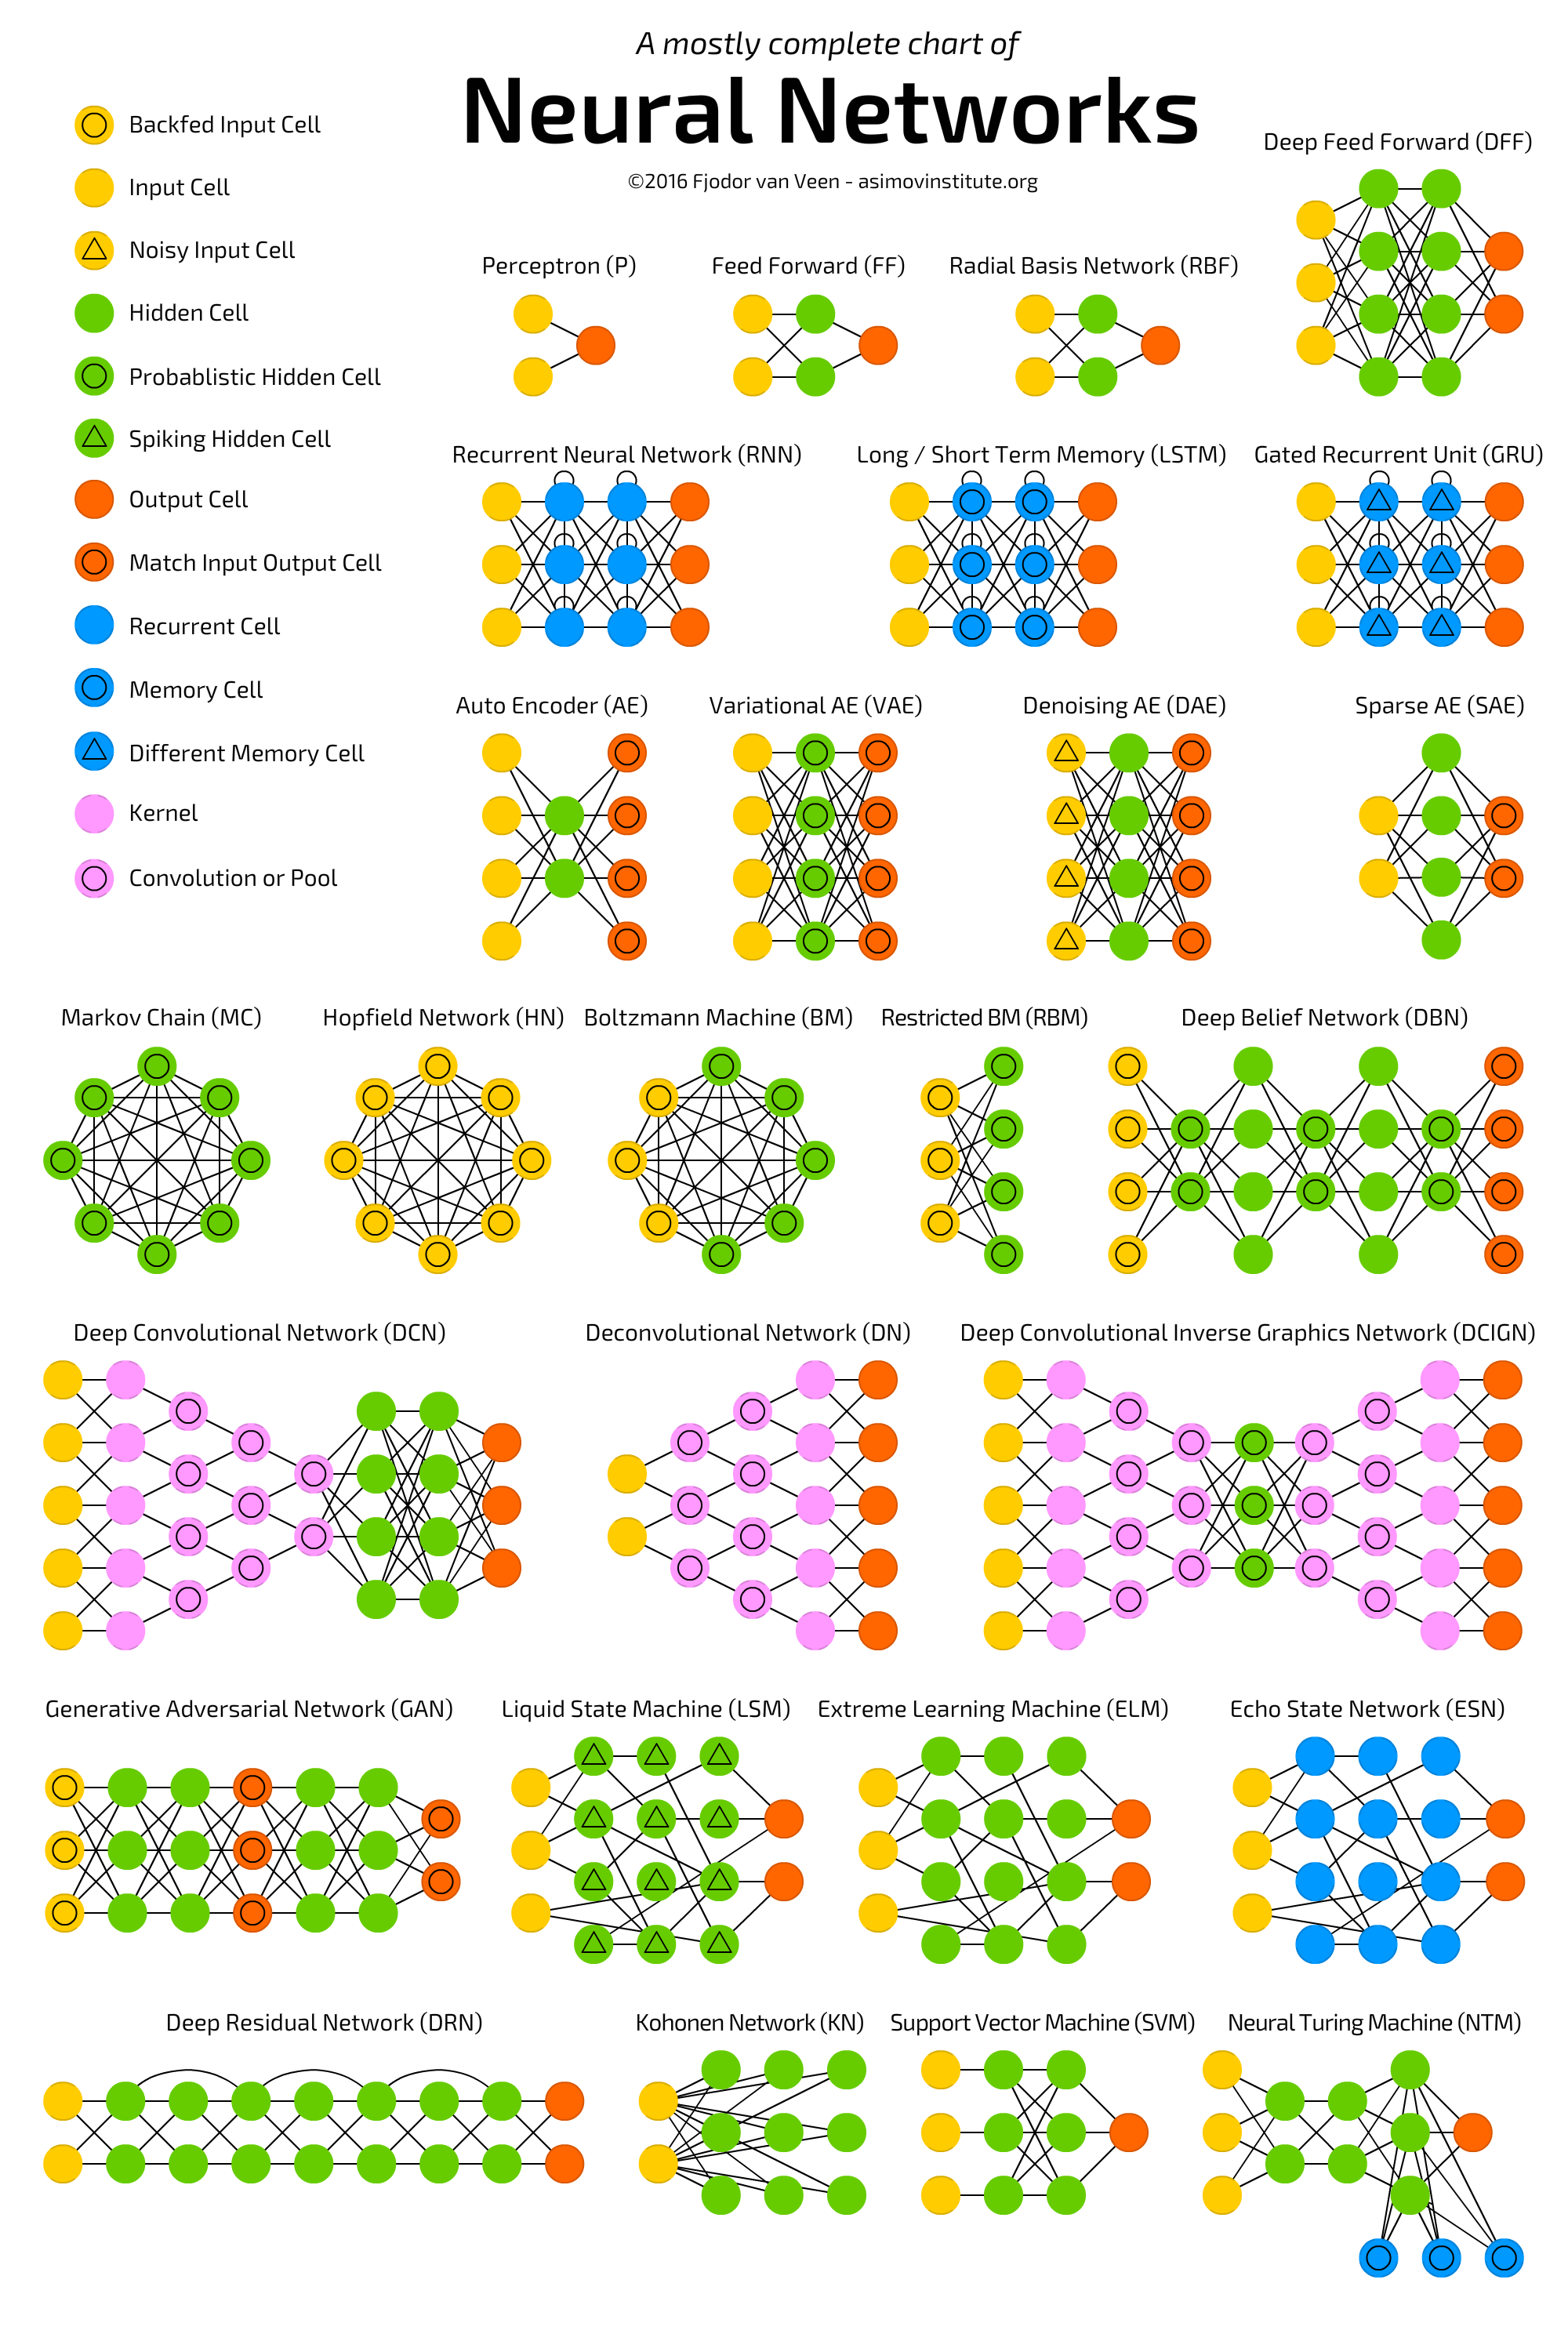
\includegraphics[width=\linewidth]{images/DifferentNN.png}
\end{figure}

\paragraph{Choosing}
There are many different options to choose from, however, the majority of them can't be used. Why? In this particular experiment, NN are being used to predict stock prices. The stock market doesn't arbitrarily choose the price every second, instead, the price is a derived from the previous prices to create a new price (it is also important to note stocks are very dependent on the news around the company). This \textit{requires} the NN to remember previous information to make informed decisions. As a result, only Recurrent Neural Networks (RNN) can be used. Something to note, GRU and LSTM are a subsection of RNN not demonstrated in the figure above.   

%http://www.wildml.com/2015/09/recurrent-neural-networks-tutorial-part-1-introduction-to-rnns/
\paragraph{RNN}
What is so special about RNN? To put it short, RNN are a special type of NN where the previous information directly affects the result of the next step in a sequential order. While in theory they are able to have arbitrarily long pieces of sequential information, a generic RNN is unable to do so. This is very bad in the context of running it on stock data as stock data can be over decades. This is why LSTM - long short term memory - are used.

%https://colah.github.io/posts/2015-08-Understanding-LSTMs/
\paragraph{LSTM}
While generic RNN struggle to remember long term information, LSTM are designed to do so making them the perfect candidate for stock market data! Below, is going to be the break down of exactly how the LSTM is able to do so.

%https://medium.com/mlreview/understanding-lstm-and-its-diagrams-37e2f46f1714
\begin{figure}[H]
  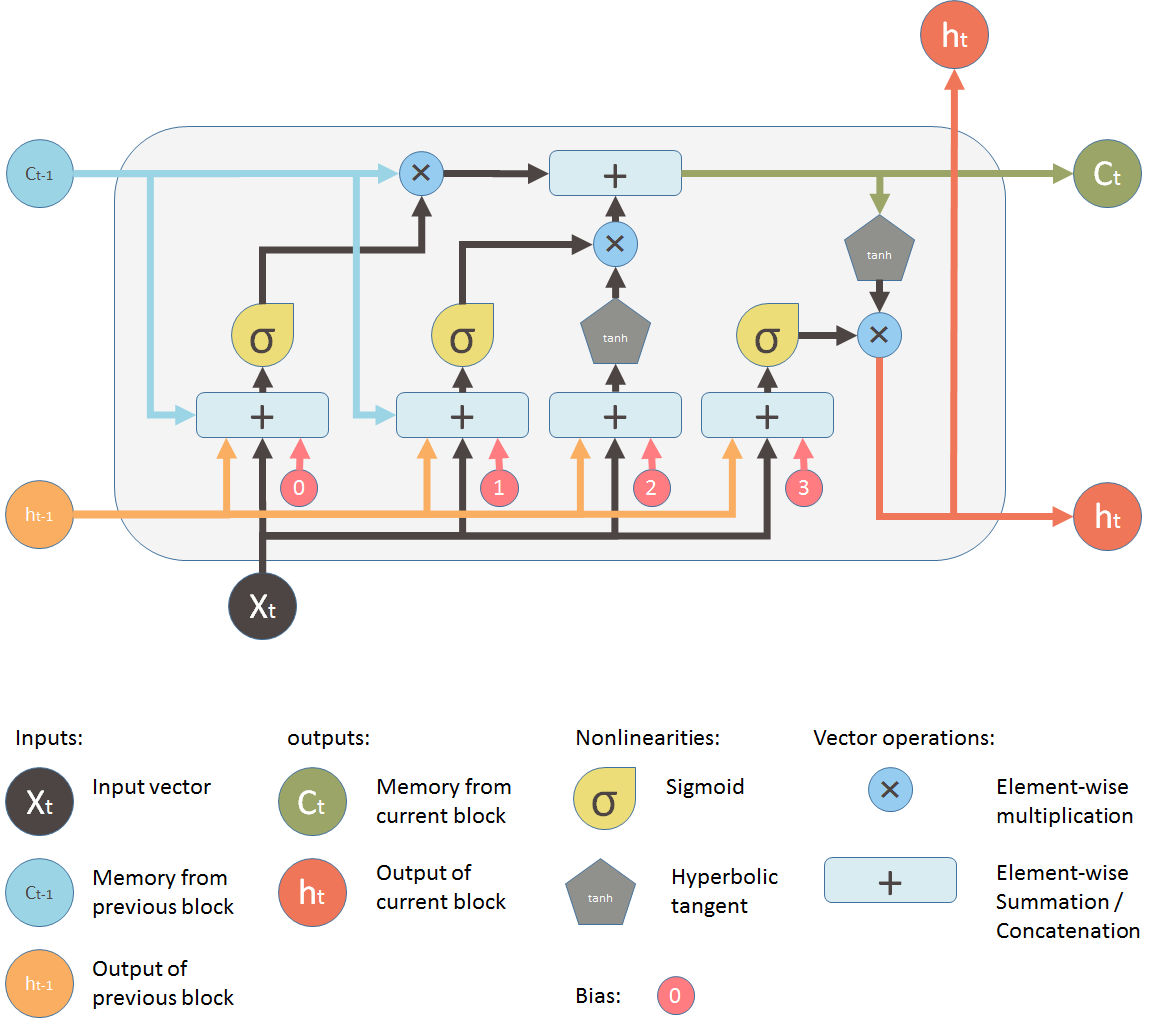
\includegraphics[width=\linewidth]{images/LSTM.png}
  \caption{Internals of LSTM cell}
\end{figure}

Although it looks very intimidating, the operations taking place are fairly straight forward. First, notice what is going in and out of this basic LSTM cell. $X_t$ is the input at the current step, $h_{t-1}$ is the output from the previous LSTM cell and $C_{t-1}$ is the ``memory'' of the previous cell. Lastly, we have $h_t$ for output of the current network and $C_t$ is the current memory of this cell. 

\begin{figure}[H]
  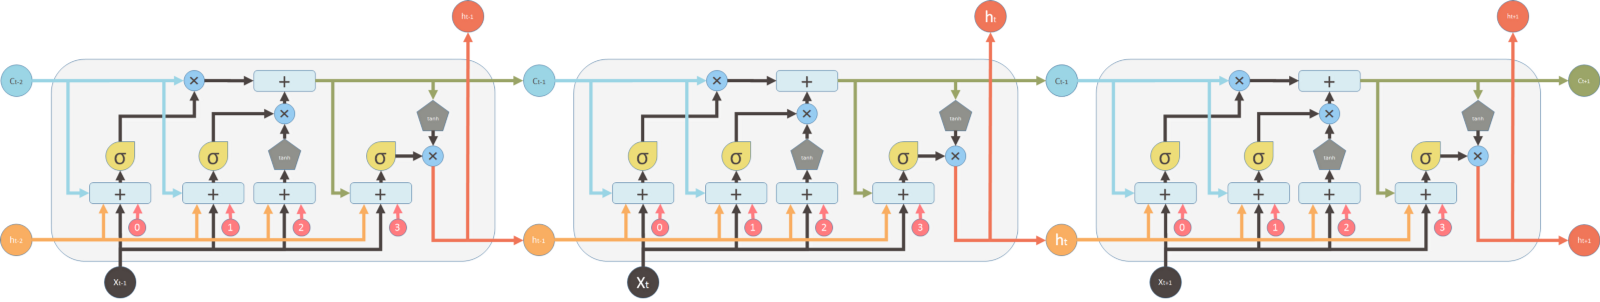
\includegraphics[width=\linewidth]{images/MultiLSTM.png}
  \caption{Multiple LSTM strung together in a chain}
\end{figure}

Here is several cells put together to visualize a segment of what is going on. The top bar ( where $C_{t-1}$ is passed) is the transfer of the memory through the network. In Figure 6 (below) we are looking at what is the ``forget'' gate. The purpose is to use a single layer NN with a sigmoid activation function which is than applied to the old memory. As a result, it can affect the memory that is continued to be passed on (which is how the network doesn't get bogged down by remembering absolutely everything). 

\begin{figure}[H]
  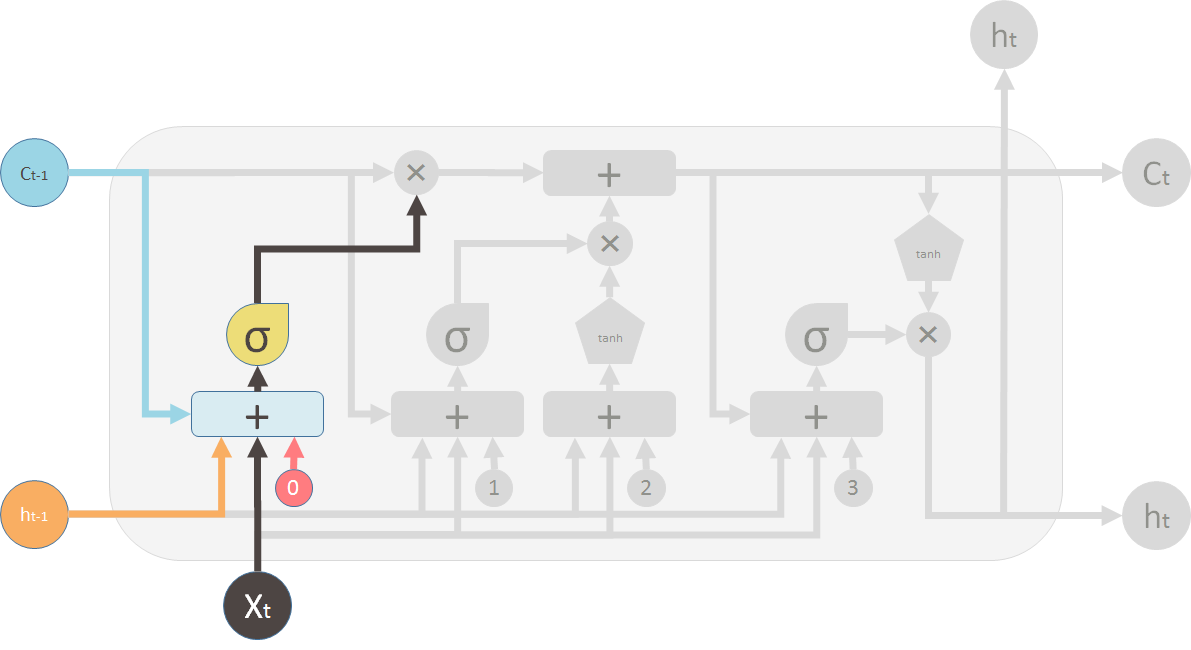
\includegraphics[width=\linewidth]{images/FirstValve.png}
  \caption{Multiple LSTM strung together in a chain}
\end{figure}

Afterwards, we go to the ``new memory'' single layer NN. This NN determines how much the new memory should influence the old memory. However, the new memory is generated by a different single layer NN, this time with $\tanh$ as the activation function. The output of both of these is combined with each other and applied to the transferring memory. 

\begin{figure}[H]
  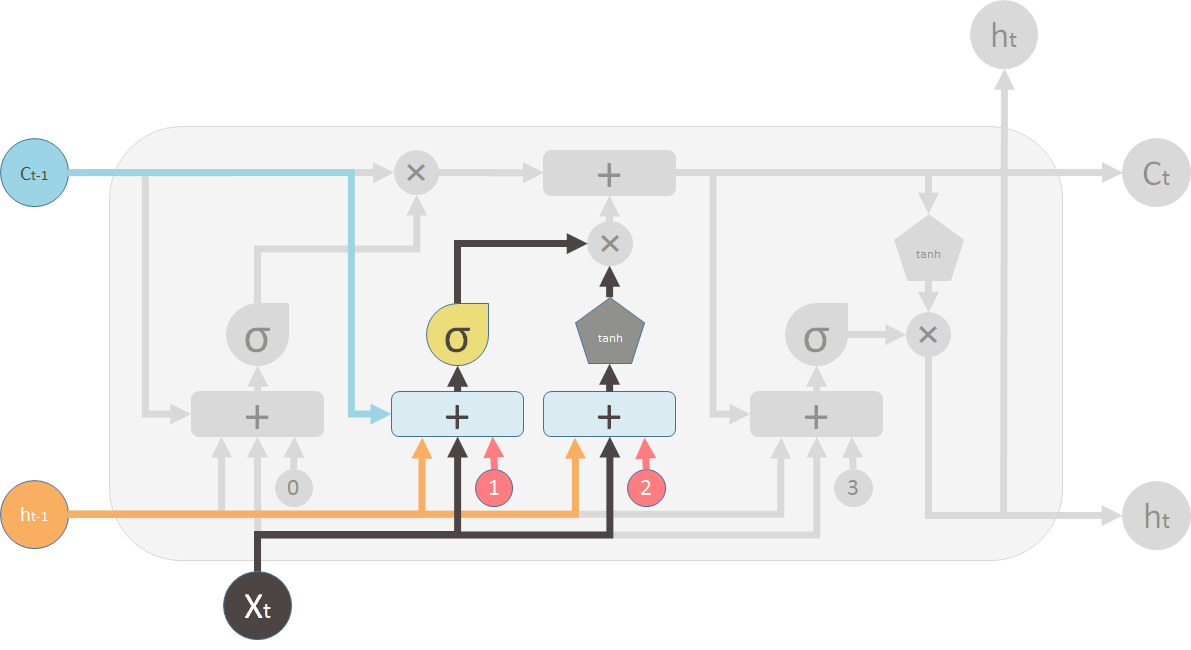
\includegraphics[width=\linewidth]{images/SecondValve.png}
  \caption{First section of LSTM}
\end{figure}

Lastly, we need to actually generate the output for this cell. This step once again includes a single layer NN that determines how much the new memory should affect the output of the cell.

\begin{figure}[H]
  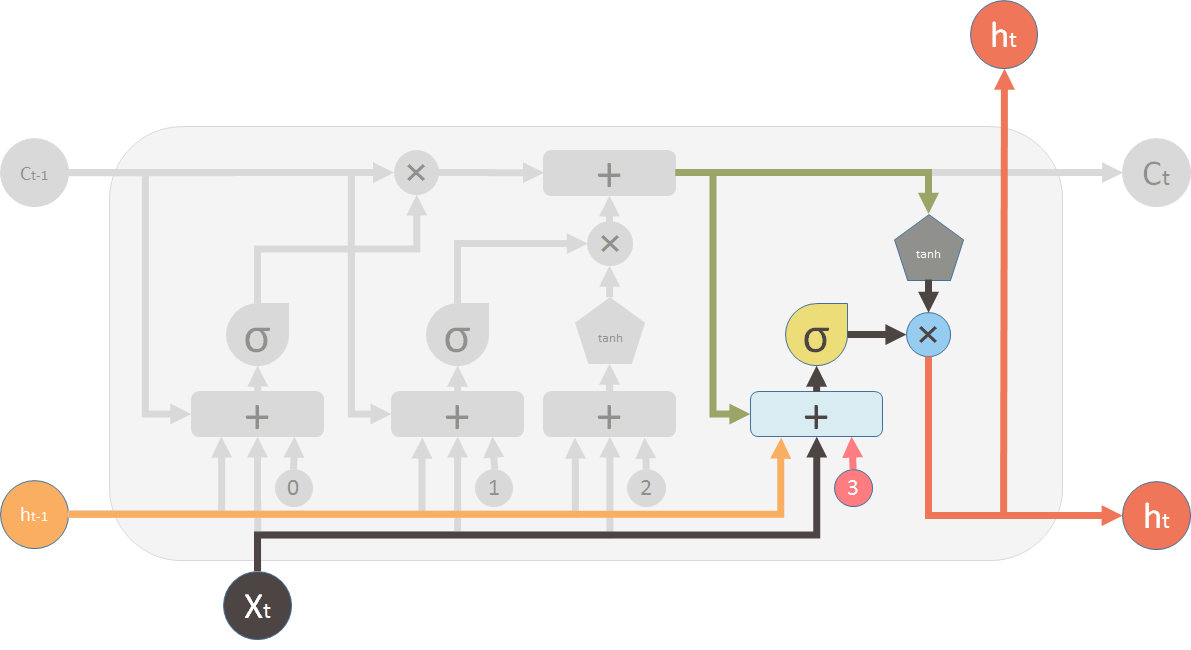
\includegraphics[width=\linewidth]{images/LastValve.png}
  \caption{Last section of LSTM}
\end{figure}

%https://medium.com/@vivek.yadav/why-dropouts-prevent-overfitting-in-deep-neural-networks-937e2543a701
\paragraph{Final Notes}
In total, because of the ability to be trained to forget unimportant information but still remember the past, it becomes the strongest RNN to use. Lastly, there is a major issue to be aware. Say we have a simple NN that we want to use to identify if we have a cat in the image. If we pass the same image to the NN over and over again, with no variation, the NN will become \textbf{overfitted}. Overfitting is simply when the NN trains to conform to the test data only so in this case, it could become perfectly accurate at knowing if that specific picture has a cat, but will be unable to determine if any other photo does accurately. One way to counter this is to use dropouts. Dropouts will drop a percentage of the data in otder to force more variability in the data being passed. Although using dropouts seem counter intuitive, especially in the case of stock markets where order matters (which will be tested), they can bring significant accuracy gains. 

\section{Setup}
Now that we have selected the RNN to use, we can go through and configure the model. All code is on github at: https://github.com/Programatic/StockMarketAI
Just a note, all code is in the form of a Jupyter notebook in vscode which allows for more modular development with data science tools. \\

\section{Results}
For the first test, the model being used is going to be LSTM $\rightarrow$ Dropout $\rightarrow$ LSTM $\rightarrow$ Dropout $\rightarrow$ LSTM $\rightarrow$ Dropout $\rightarrow$ LSTM $\rightarrow$ Dropout $\rightarrow$ Dense. The dense layer just takes the information from the previous layers and condenses it to a dimension we want, in this case 1 (as in 1 output value for the price of the stock). \\
Here is a graph of McDonalds stock from 1970. The training set is going to be the first $\frac{1}{3}$ of the stock and the test will be the rest. 
\begin{figure}[H]
  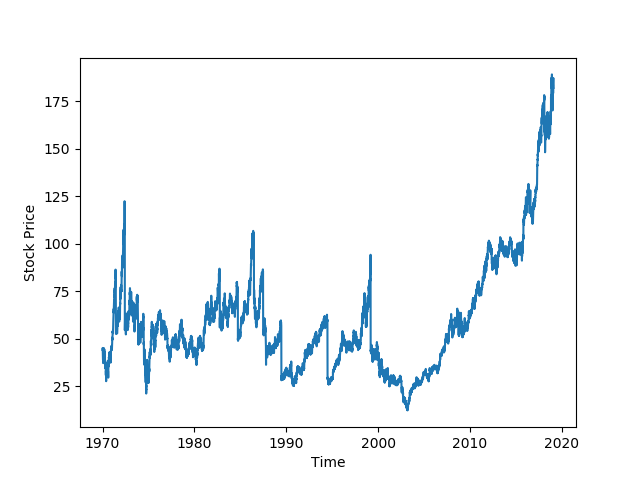
\includegraphics[width=\linewidth]{images/graph1.png}
  \caption{McDonalds Stock}
\end{figure}

\section{Conclusions}\label{conclusions}
We worked hard, and achieved very little.

\bibliographystyle{abbrv}
\bibliography{main}

%https://www.sas.com/en_us/insights/analytics/what-is-artificial-intelligence.html

\end{document}
